Up until this chapter most of the experiments are done in 1Gbps network environments.
The proposed load balancers have shown decent performance levels in 1Gbps environment.
However, it is essential to investigate the feasibility of the proposed load balancers in 10Gbps network environments.
In this chapter, the author carries out throughput measurements of ipvs-nat, ipvs-tun, and iptables DNAT in 10Gbps environment.
Then the author improves the performance levels of ipvs-nat and ipvs-tun by setting up these load balancers in the node net namespace.
Also presented is the novel software load balancer using eXpress Data Plane(XDP) technology, as an alternative to ipvs software load balancers.

\section{Throuput of ipvs-nat, ipvs-tun and iptables DNAT}

Figure~\ref{fig:bench_10g} shows the packte flow for ipvs-nat and iptables DNAT, and Figure~\ref{fig:bench_10g_l3dsr} shows that for ipvs-tun.
The 10Gbps NICs are used for benchmark client and the node for the load balancer.
In the case of the ipvs-nat and iptables DNAT, the response packets from nginx pods are returned to the load balancer, and then load balancer returns it to the client.
In contrast, in the case of ipvs-tun, the response packets from nginx pods are directly returned to the client.
Since the load balancer does not have to process the response packet, the better performance level is expected for ipvs-tun.

\begin{figure}[h]
  \centering
  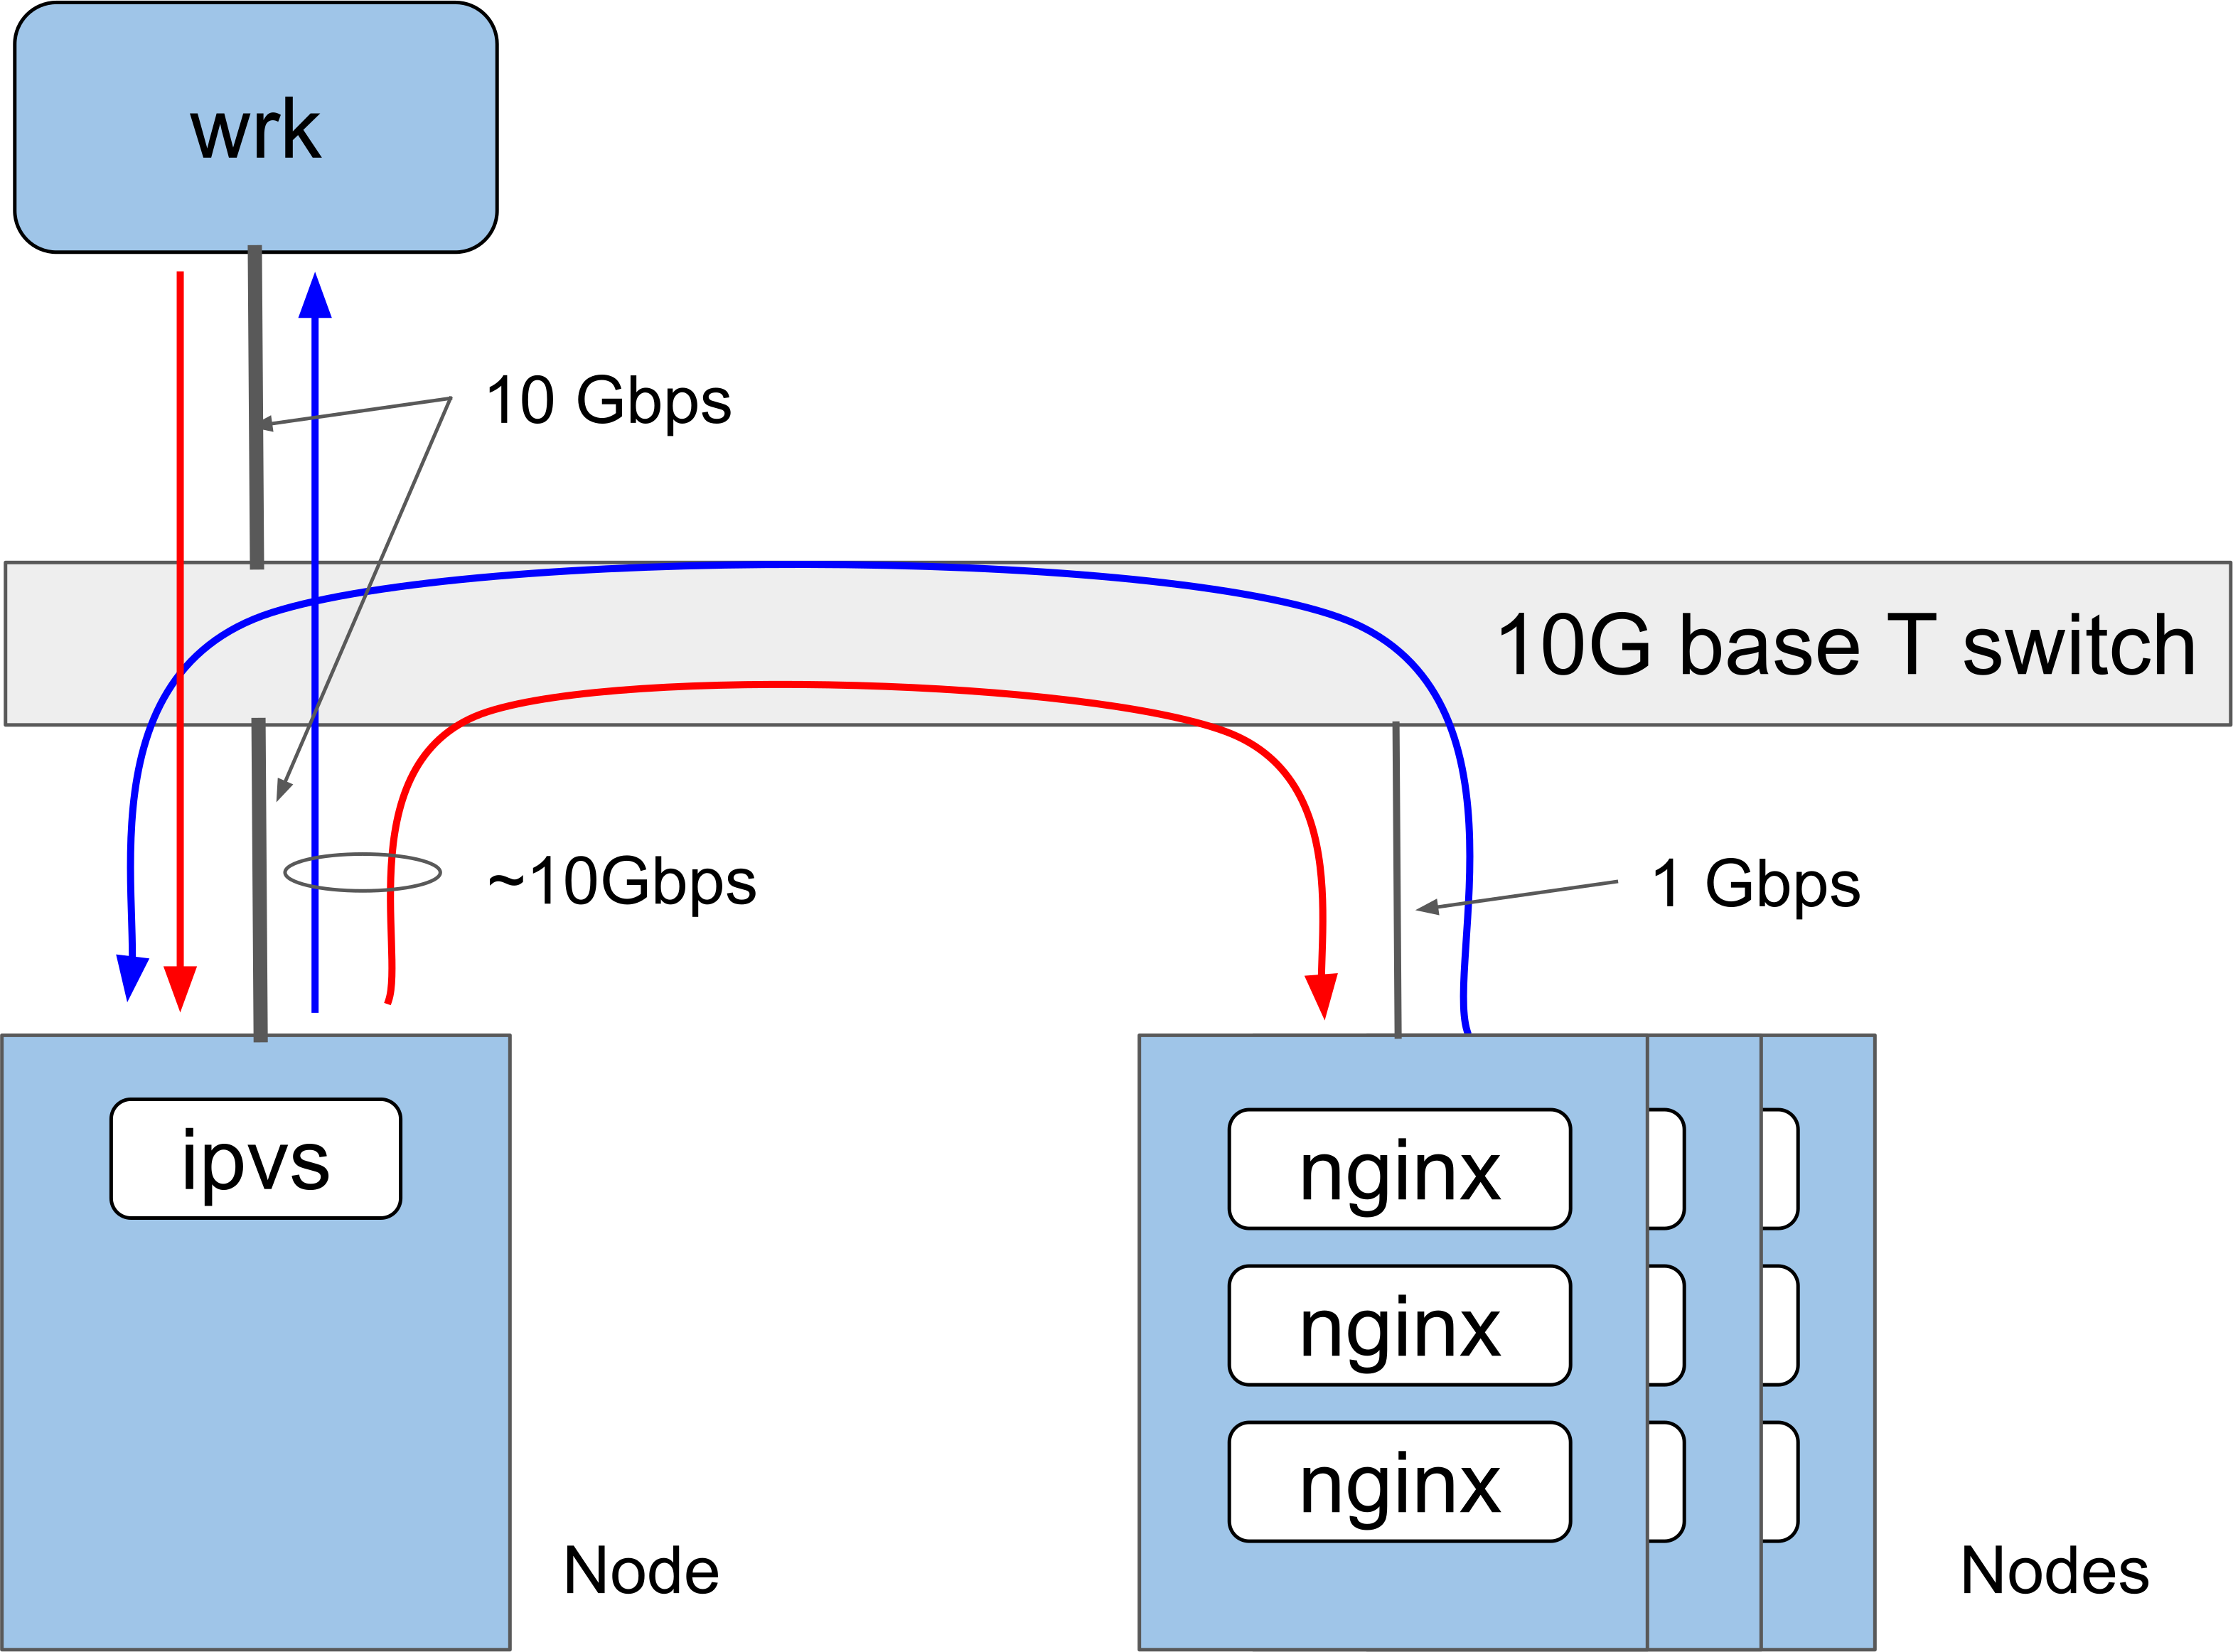
\includegraphics[width=0.8\columnwidth]{Figs/bench_10g}
  \caption{Packet flow of ipvs-nat and iptables DNAT.}
  \label{fig:bench_10g}
\end{figure}

\begin{figure}[h]
  \centering
  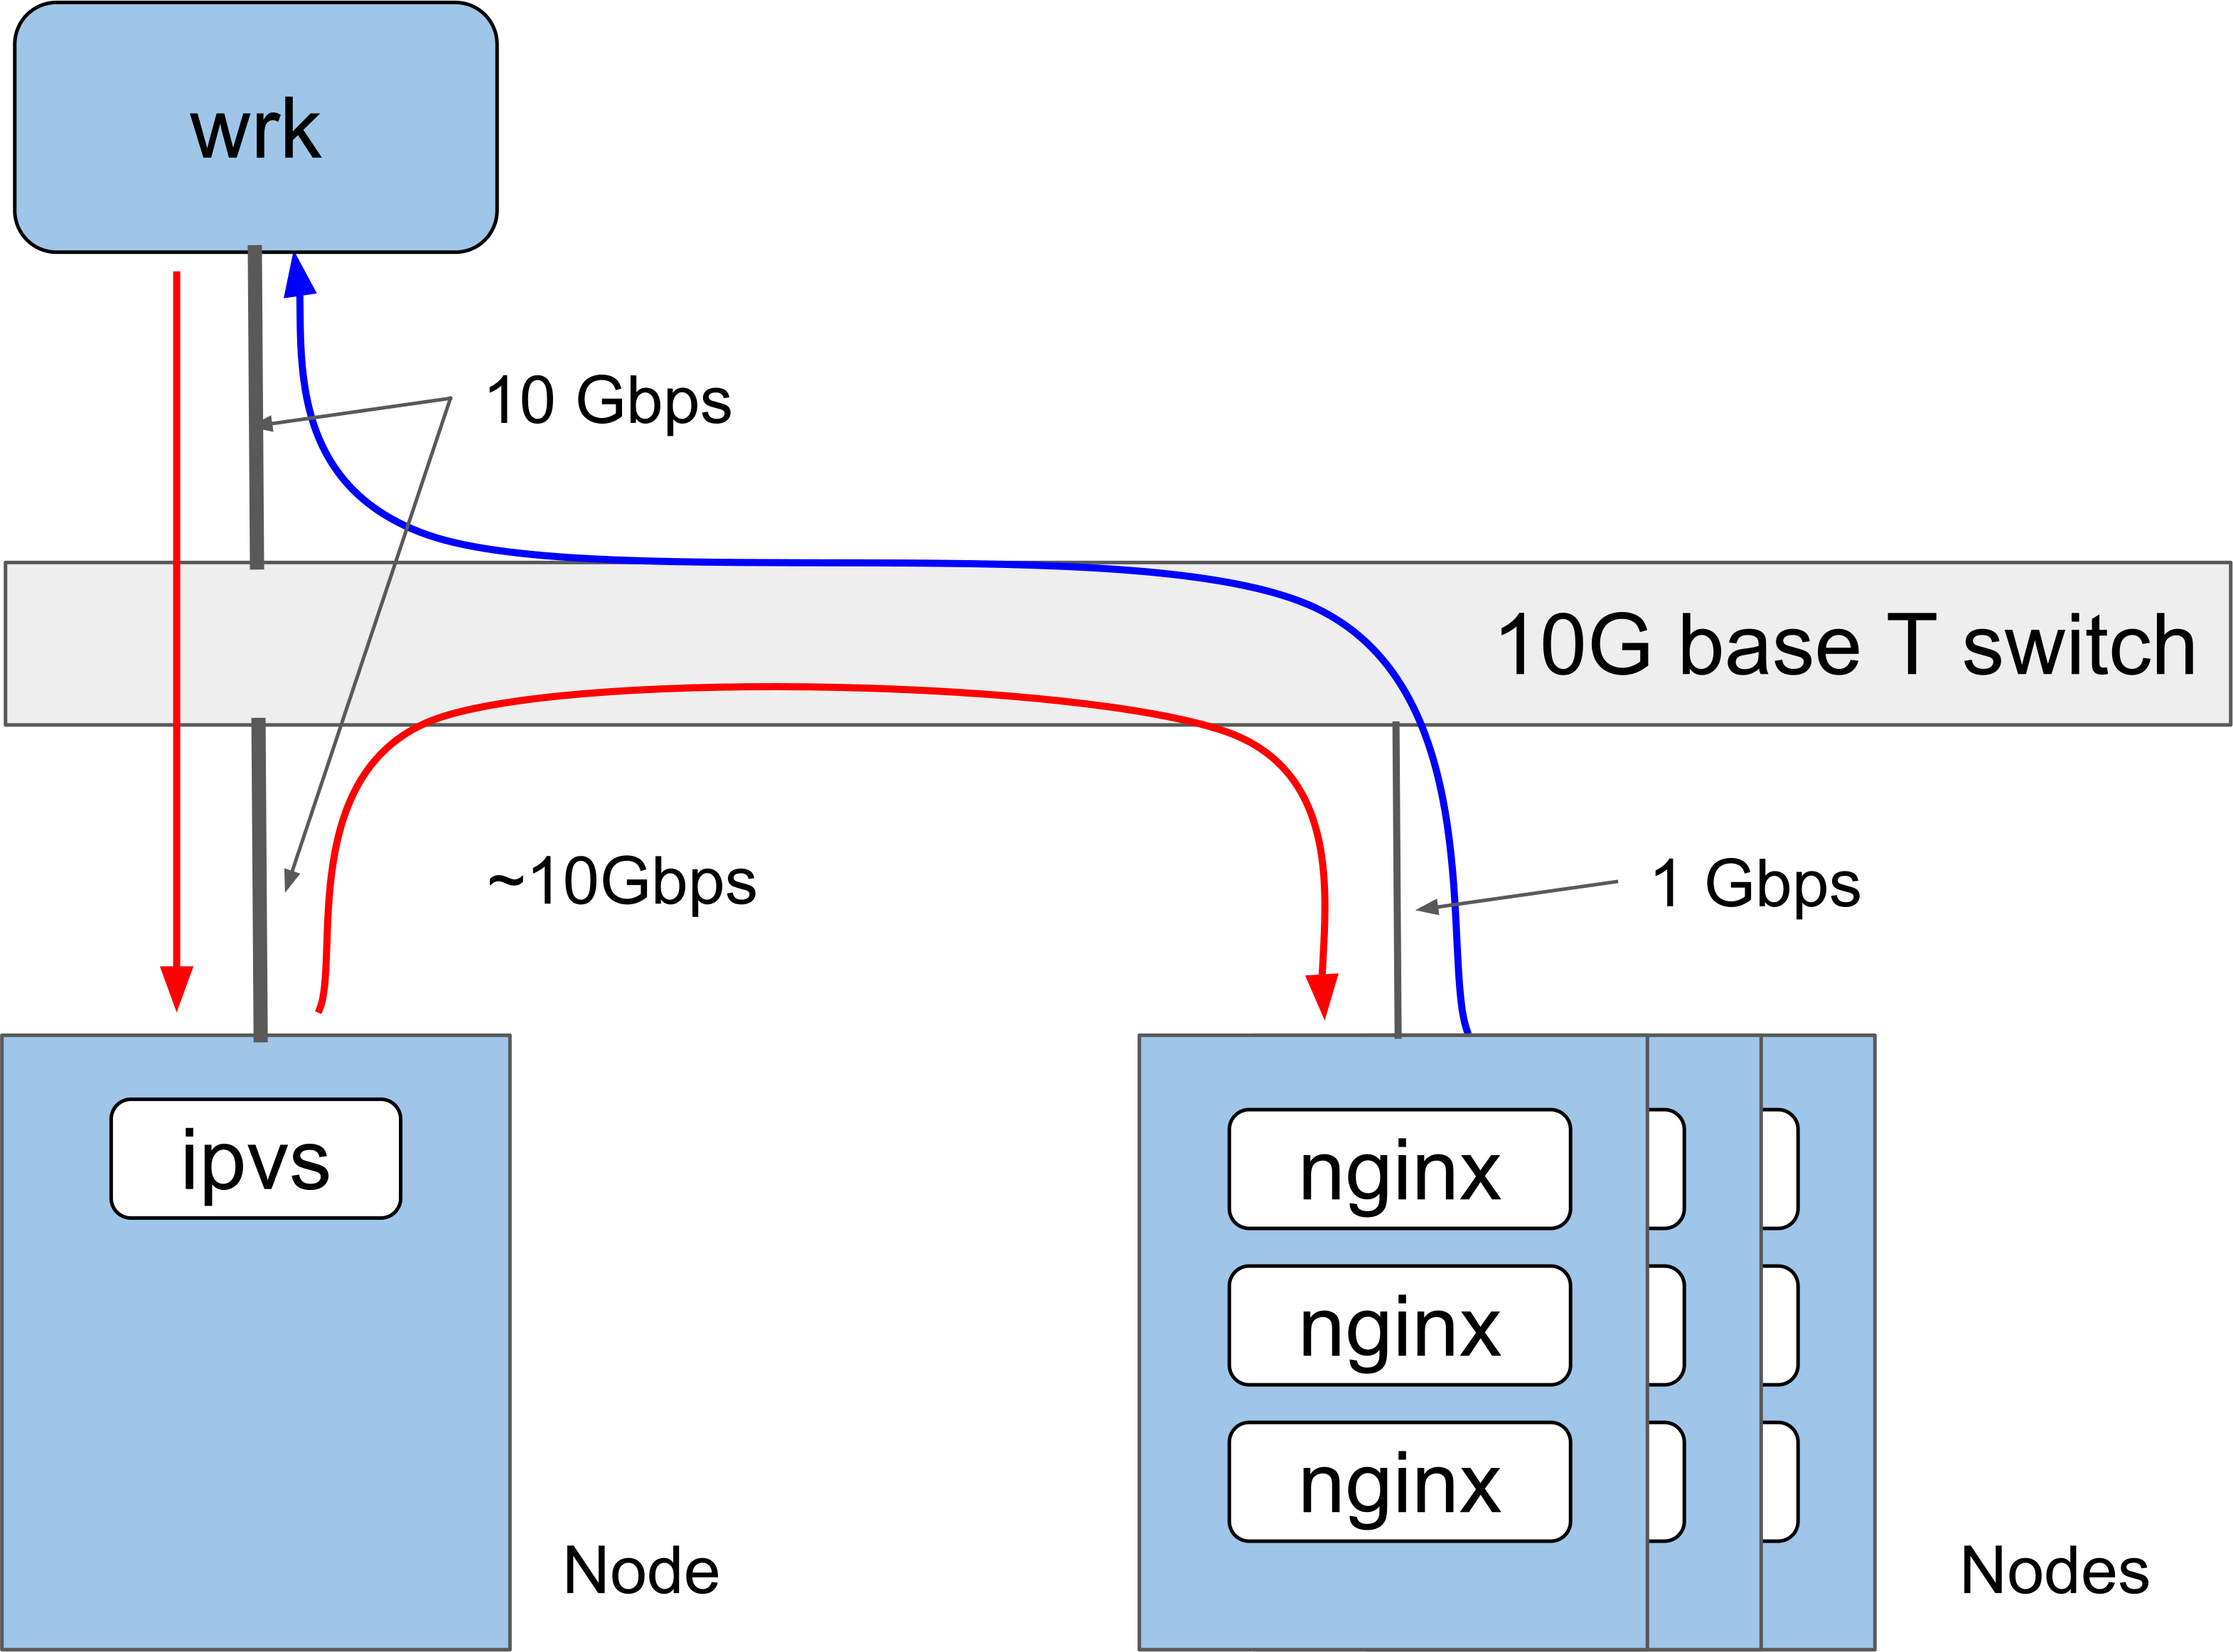
\includegraphics[width=0.8\columnwidth]{Figs/bench_10g_l3dsr}
  \caption{Packet flow of ipvs-tun.}
  \label{fig:bench_10g_l3dsr}
\end{figure}

\begin{figure}[h]
  \centering
  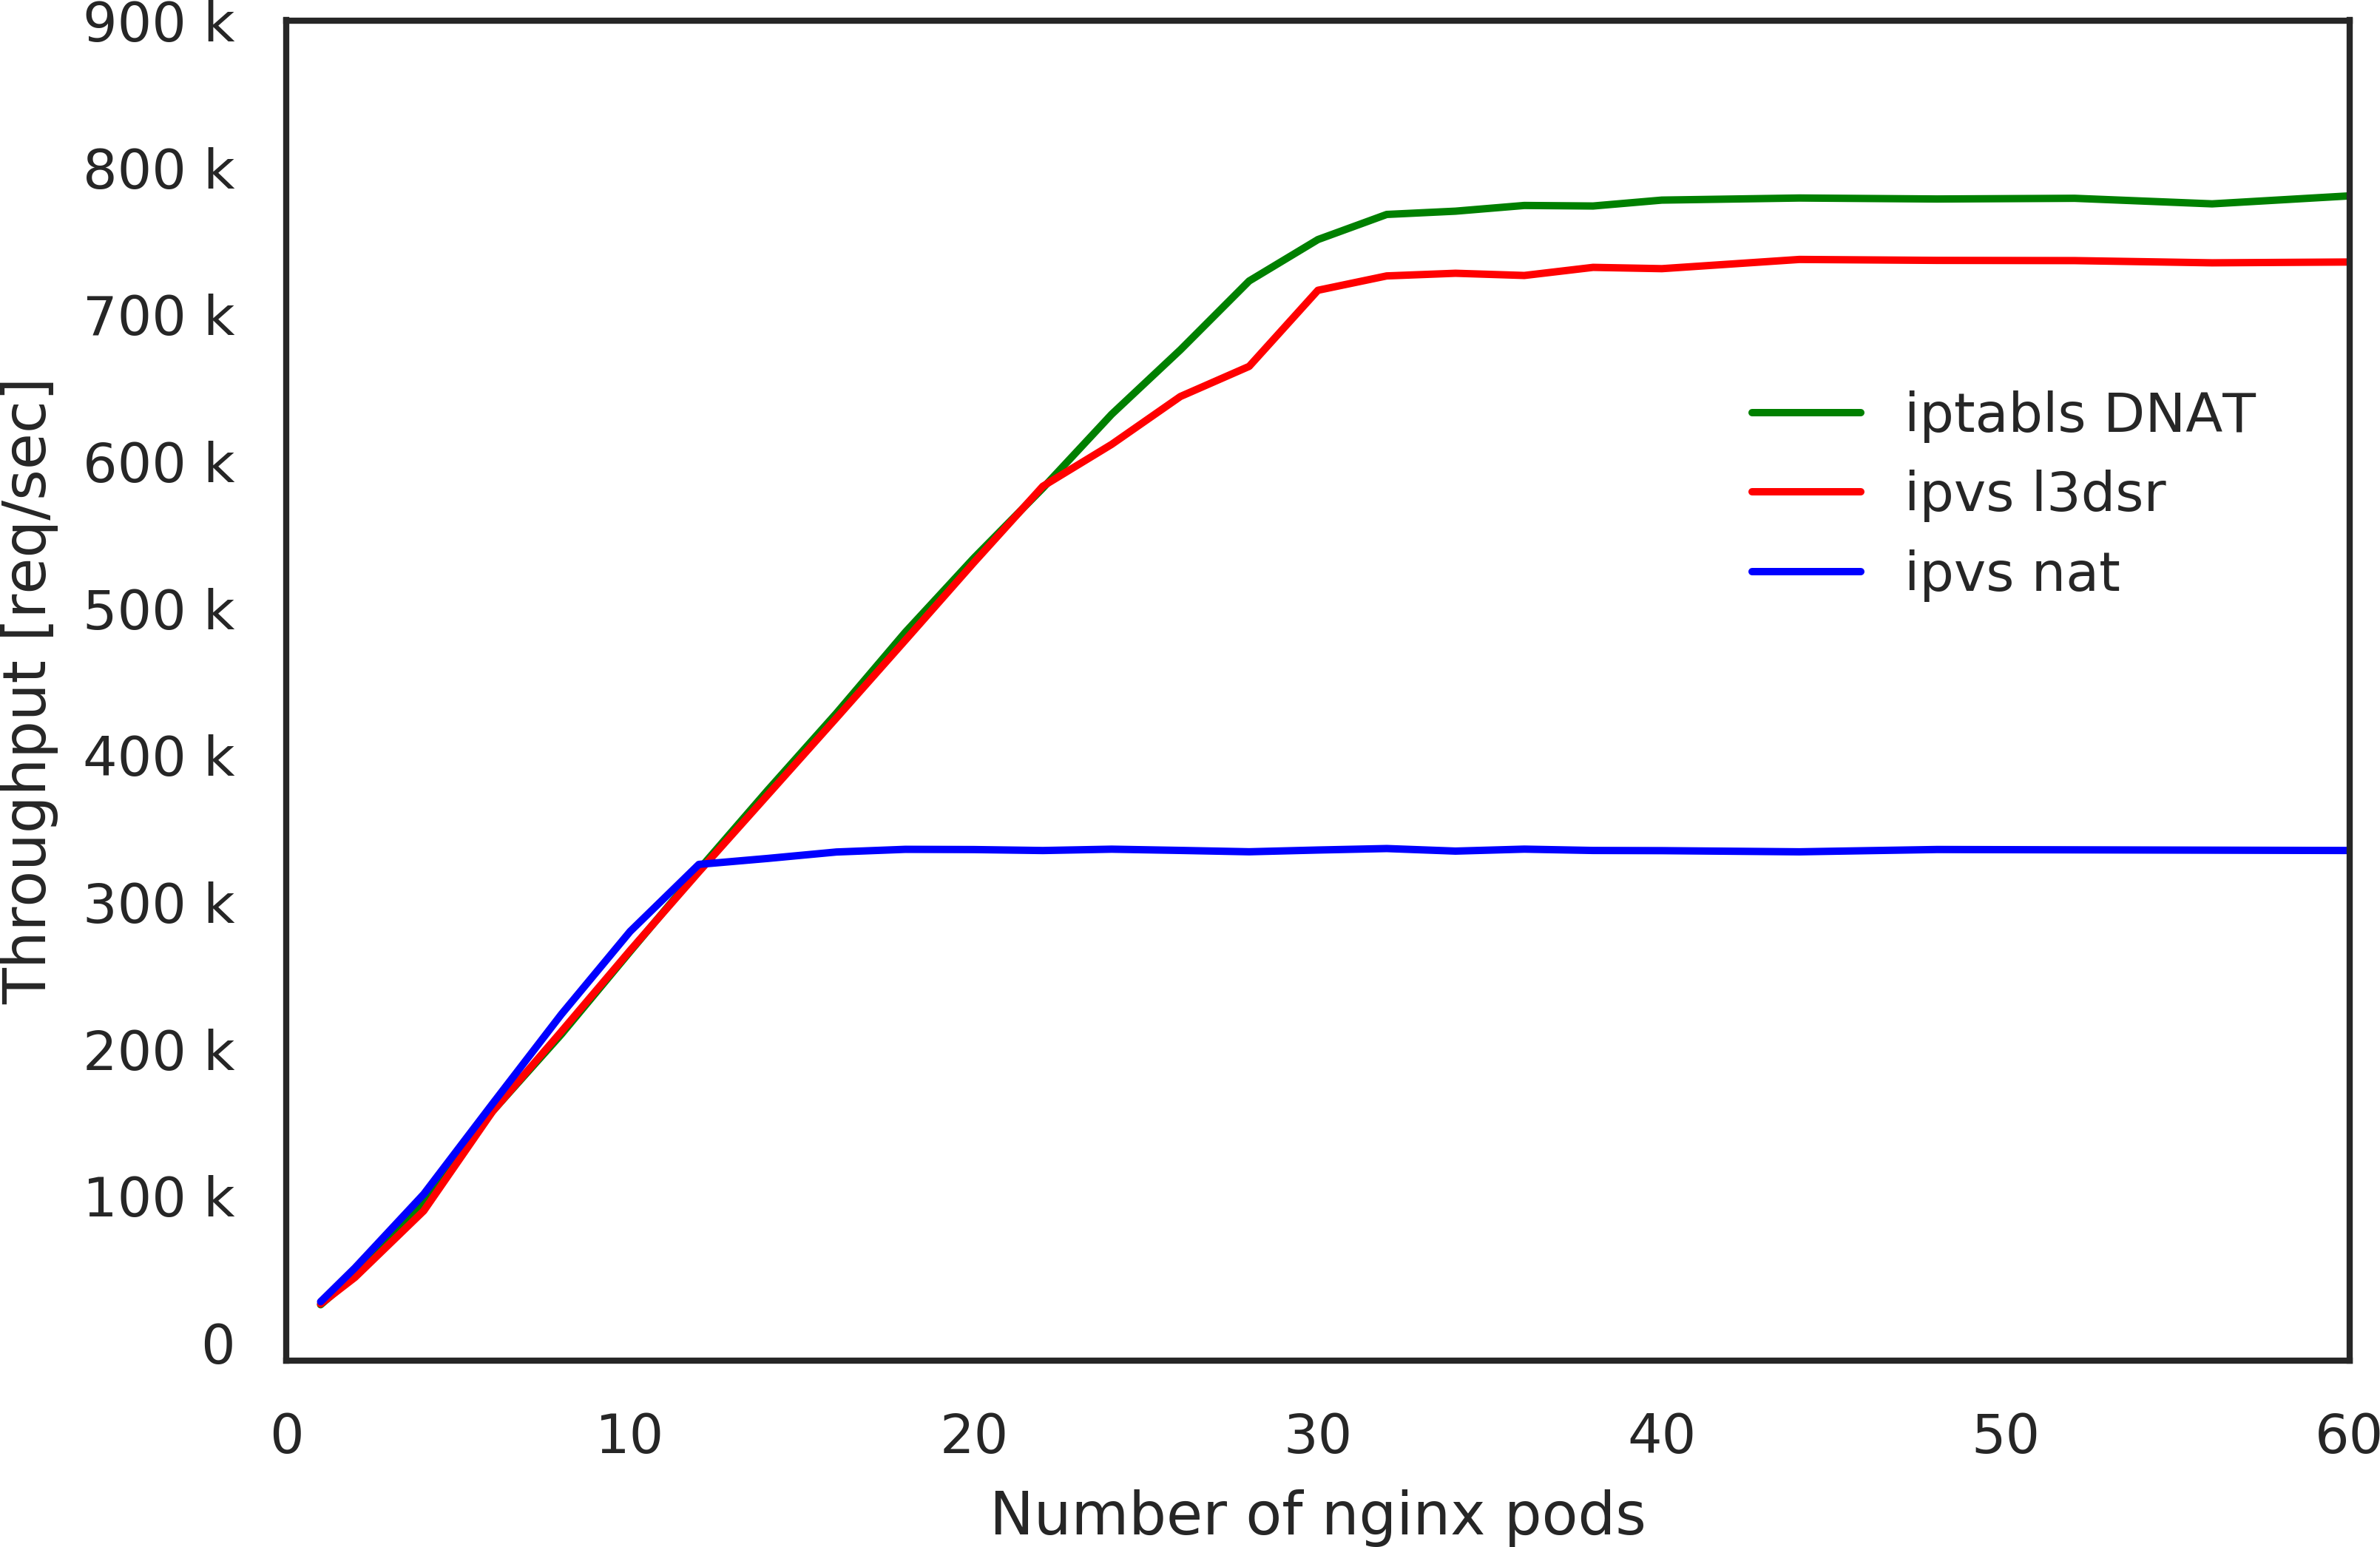
\includegraphics[width=0.8\columnwidth]{Figs/ipvs_l3dsr_10g}
  \caption{Throughput of load balancers in 10 Gbps.}
  \label{fig:ipvs_l3dsr_10g}
\end{figure}

Figure~\ref{fig:ipvs_l3dsr_10g} shows the throughput of ipvs-tun, ipvs-nat and iptables DNAT in 10Gbps environment.
We can see the general characteristics of a load balancer where the throughput increases linearly to a certain level as the number of nginx container increases, and then eventually saturates.
These saturation levels are the performance limits of each of the load balancers, which is determined by packet forwarding efficiency or the bandwidth of the network.
The performance limit of the iptables DNAT is close to 780k [req/sec], where the CPU usage of the benchmark client becomes 100\%.

Table~\ref{table:nat_tun_dnat_1g_10g} summarizes the throughput of ipvs-tun, ipvs-nat and iptables DNAT at 40 nginx pods in 10 Gbps and 1 Gbps networks.
By using 10 Gbps network, the performance levels for all of these load balancer are improved.
However, the magnitudes of the improvements are different among the types of the load balancers.
While the throughput of the ipvs-nat is 334833 [req/sec], that of the iptables DNAT is 777640 [req/sec].
This suggests that the packet forwarding of the iptables DNAT is more efficient than that of ipvs-nat.
Although the throughput of the ipvs-tun, 730975 [req/sec] is better than ipvs-nat because of the L3DSR settings, it still falls short of that of iptables DNAT.
It seems that containerized ipvs load balancers are inherently less efficient than the iptables DNAT, which could be attributed to either overhead of container network(veth+bridge) or kernel code for ipvs itself.
In order to investigate this issue, the author conducted a throughput measurement for ipvs-nat and ipvs-tun that are set up in node net namespaces in the next section.

\begin{table}[H]
  \centering
  \begin{tabular}{|l|r|r|}
    \hline
    & \multicolumn{2}{c|}{Throughput {[}req/sec{]}} \\ \hline
    Type of load balancer & \multicolumn{1}{c|}{1Gbps} & \multicolumn{1}{c|}{\cellcolor[HTML]{ECF4FF}10Gbps} \\ \hline
    \multicolumn{1}{c|}{iptables DNAT} & 193198 & \cellcolor[HTML]{ECF4FF}777640 \\ \hline
    \multicolumn{1}{c|}{ipvs-nat} & 195666 & \cellcolor[HTML]{ECF4FF}334833 \\ \hline
    \multicolumn{1}{c|}{ipvs-tun} & 292660 & \cellcolor[HTML]{ECF4FF}730975 \\ \hline
  \end{tabular}
  \caption{Performance levels in 1Gbps and in 10Gbps.}
  \raggedright
  Throughput results of the load balancers at 40 nginx pods from the data for the Figures~\ref{fig:ipvs_l3dsr_1g.png} and \ref{fig:ipvs_l3dsr_10g} are shown.
  \label{table:nat_tun_dnat_1g_10g}
\end{table}

\FloatBarrier
\section{Throuput of ipvs-nat, ipvs-tun and iptables DNAT}

In order to improve the throughput of the ipvs load balancers by removing the overhead of container network, the ipvs load balancers were set up in node net namespaces.
Appendix XXX shows inside of ipvs container script that launches the keepalived in node net namespaces.
By doing so, the load balancing tables are created in the node net namespace.

Figure~\ref{fig:ipvs_node_l3dsr_10g} shows the throughput of ipvs-nat and ipvs-tun in the node namespace together with the throughput of the iptables DNAT.
The throughput of the ipvs-tun is almost identical to that of iptables DNAT, which is limited by CPU power of the benchmark client. 
%
Although the throughput of the ipvs-nat is smaller than that of the iptables DNAT, it is clearly improved from the result in Figure~\ref{fig:ipvs_l3dsr_10g}.

Table~\ref{table:nat_tun_dnat_pod_node} compares the throughput of ipvs load balancers in the pod namespace and in the node namespace at 40 nginx pods.
The thoughput data are taken from the results in the Figures~\ref{fig:ipvs_l3dsr_10g} and \ref{fig:ipvs_node_l3dsr_10g}.
We can see that maximum throughputs can be improved in the case of load balancers in node namespace both for the ipvs-nat and the ipvs-tun.  

\begin{figure}[h]
  \centering
  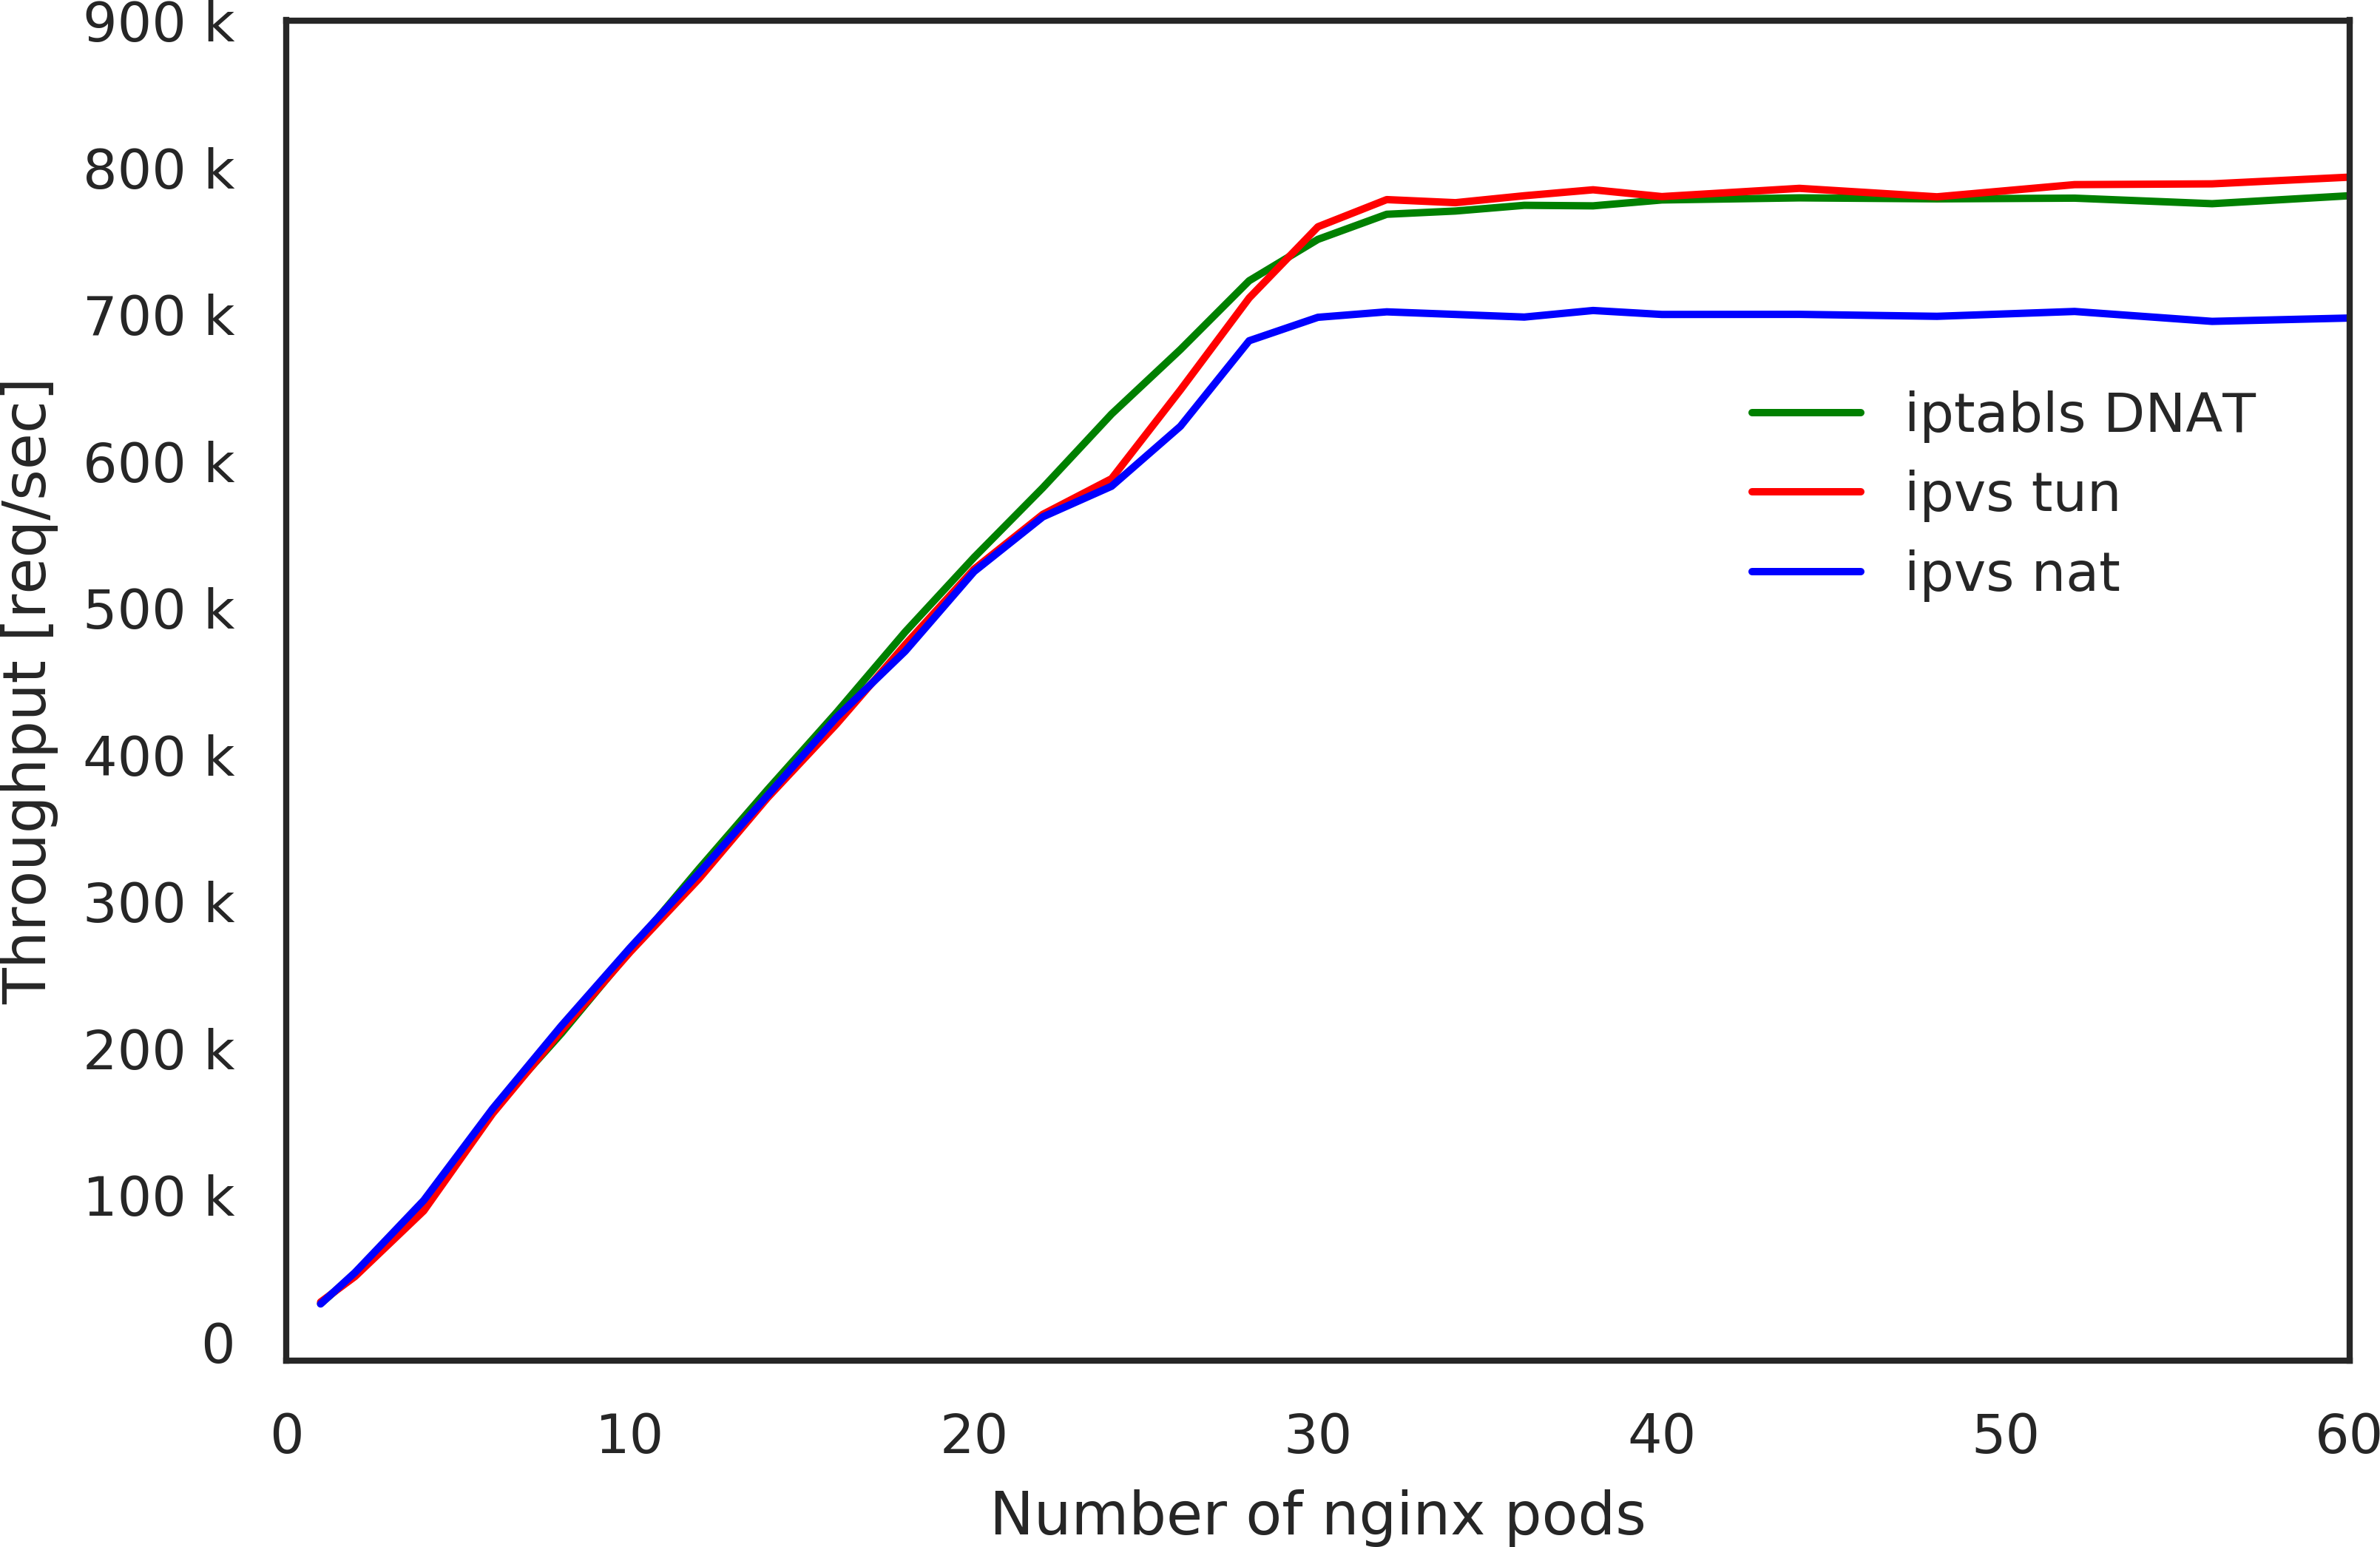
\includegraphics[width=0.8\columnwidth]{Figs/ipvs_node_l3dsr_10g}
  \caption{Throughput of load balancers in node name space.}
  \label{fig:ipvs_node_l3dsr_10g}
\end{figure}

\begin{table}[h]
  \centering
  \begin{tabular}{|l|r|r|}
    \hline
    & \multicolumn{2}{c|}{Throughput {[}req/sec{]}} \\ \hline
    Type of load balancer & \multicolumn{1}{c|}{pod name space} & \multicolumn{1}{c|}{node name space} \\ \hline
    \multicolumn{1}{c|}{iptables DNAT} & NA & \cellcolor[HTML]{ECF4FF}777640 \\ \hline
    \multicolumn{1}{c|}{ipvs-nat} & \cellcolor[HTML]{ECF4FF}334833 & \cellcolor[HTML]{FFF3F3}699635 \\ \hline
    \multicolumn{1}{c|}{ipvs-tun} & \cellcolor[HTML]{ECF4FF}730975 & \cellcolor[HTML]{FFF3F3}779932 \\ \hline
  \end{tabular}
  \caption{Performance levels in pod namespace and in node namespace.}
  \raggedright
  Throughput results of the load balancers at 40 nginx pods from the data for the Figures~\ref{fig:ipvs_l3dsr_10g} and \ref{fig:ipvs_node_l3dsr_10g} are shown.
  \label{table:nat_tun_dnat_pod_node}
\end{table}

\FloatBarrier
\section{XDP load balancer}

\section{Summary}

In this chapter, the author carried out throughput measurements of ipvs-nat, ipvs-tun, and iptables DNAT in 10Gbps environment.
From the results the general characteristics of a load balancer are observesd.
The throughput increases linearly to a certain level as the number of nginx container increases, and then eventually saturates.
The performance levels for of the load balancers are improved by using 10Gbps network.
However, the throughputs of ipvs-nat and ipvs-tun are smaller than that of iptables DNAT.

Then the author improved the performance levels by setting up ipvs-nat and ipvs-tun load balancers in the node net namespace to remove overhead of the container network.
The throughput of the ipvs-tun became almost identical to that of iptables DNAT, and the throughput of the ipvs-nat also improved to the level close to that of the iptables DNAT.

The authot also presented the novel software load balancer using eXpress Data Plane(XDP) technology, as an alternative to ipvs software load balancers.
And brah brah brah.....



